%%%%%%%%%%%%%%%%%%%%%%%%%%%%%%%%%%%%%%%%%%%%%%%%%%%%%%%%%%%%%%%%%%%%%%%%
%%% PAKDD 2026 Paper - CMAS4G2
%%%%%%%%%%%%%%%%%%%%%%%%%%%%%%%%%%%%%%%%%%%%%%%%%%%%%%%%%%%%%%%%%%%%%%%%
\documentclass[runningheads]{llncs}
\usepackage[T1]{fontenc}
\usepackage{booktabs}
\usepackage{graphicx}
\usepackage{amsmath}
\usepackage{amsfonts}
\usepackage{amssymb}
\usepackage{array}
\usepackage{multirow}
\usepackage[table]{xcolor}
\usepackage{url}
\usepackage{hyperref}
\usepackage{minted}
%%%%%%%%%%%%%%%%%%%%%%%%%%%%%%%%%%%%%%%%%%%%%%%%%%%%%%%%%%%%%%%%%%%%%%%%
\begin{document}
% \title{CMAS4G2: A Cooperative Multi-Agent System for Gherkin Acceptance Test Generation}
%\title{Locally Deployed Multi-Agent Systems for Gherkin Acceptance Test Automation}
\title{CMAS4G2: \\A Locally Deployed Cooperative Multi-Agent System for Gherkin Acceptance Test Generation}
% \author{Anonymous Author(s)}
% \authorrunning{Anonymous}
% \institute{Anonymous Institution}
% \iffalse
% \author{Arthur Pendragon\inst{1} \and Nimue\inst{2}}
% \authorrunning{A. Pendragon and Nimue}
% \institute{Camelot Castle, Camelot, United Kingdom\\
% \email{king.arthur@camelot.uk} \and
% The Lady's Lake, Avalon, United Kingdom\\
% \email{lady.of.the.lake@avalon.uk}}


\author{
    Donghao Huang\inst{1,2} \and 
    Shila Chew\inst{3} \and 
    Zhaoxia Wang\inst{1}
    \thanks{Corresponding author: zxwang@smu.edu.sg}
}
\authorrunning{D. Huang, S. Chew and Z. Wang}
\institute{
School of Computing and Information Systems, Singapore Management University, Singapore, Singapore\\
\email{dh.huang.2023@engd.smu.edu.sg, zxwang@smu.edu.sg}
\and
Research and Development, Mastercard, Arlington, VA, USA\\
\email{donghao.huang@mastercard.com}
\and
Research and Development, Mastercard, Singapore, Singapore\\
\email{shila.chew@mastercard.com}
}

% \fi

\maketitle
\begin{abstract}
Acceptance test automation remains a persistent bottleneck in software engineering, as translating natural-language requirements into executable specifications demands extensive expertise and manual effort. While large language models (LLMs) show promise in code generation, their integration into Behavior-Driven Development (BDD) pipelines---particularly for Gherkin test authoring---remains underexplored.
We introduce \textbf{CMAS4G2}, a \emph{Cooperative Multi-Agent System for Gherkin Generation} built on Microsoft's AutoGen Swarm framework. CMAS4G2 coordinates specialized Validator, Quality-Assurance, and Supervisor agents to automate requirement validation and acceptance-test synthesis. Generated artifacts are evaluated at scale using the LLM-as-a-Judge (LAJ) framework~\cite{huang2025laj}, which provides rubric-driven, automated coverage assessment aligned with expert human judgments.
Experiments on a 200-ticket benchmark derived from the Kill Bill platform show that open-weight models deployed locally on consumer hardware approach proprietary performance: %GPT-OSS 20B attains 87.6\% overall success and 85.4\% coverage versus Claude Sonnet 4's 90.4\% and 91.6\%.
% FIX 1
GPT-OSS 20B (medium reasoning, our best-performing open-weight configuration by overall success) attains 87.6\% overall success and 85.4\% coverage versus Claude Sonnet 4's 90.4\% and 91.6\%. The low-reasoning variant achieves marginally higher coverage (85.7\%) at slightly lower overall success (86.6\%).
These results demonstrate the feasibility of the proposed CMAS4G2, showing that cooperative, open-weight LLM agents can deliver competitive acceptance-test automation without cloud dependence, enabling cost-efficient, privacy-preserving quality assurance.
\end{abstract}
\keywords{Multi-Agent Systems \and Acceptance Testing \and Gherkin \and Large Language Models \and Behavior-Driven Development}

\section{Introduction}
Automated acceptance testing remains difficult: translating high-level requirements into executable tests demands domain expertise, sustained effort, and careful maintenance~\cite{zhao2020nlp4re}. Traditional tools struggle to bridge the semantic gap between natural-language requirements and testable specifications~\cite{das2024extracting}. Large language models (LLMs) show promise in code generation and semantic translation, but their application to Behavior-Driven Development (BDD)--particularly Gherkin--is underexplored~\cite{wang2024effectiveness}.
In order to address these gaps, we propose CMAS4G2, a \emph{Cooperative Multi-Agent System for Gherkin Generation}. CMAS4G2 uses Microsoft's AutoGen Swarm~\cite{autogen_swarm_docs} to coordinate specialized agents for requirement validation, test generation, and quality assurance, enforcing structured handoffs and internal checks. To measure outcome quality at scale, we adopt the \emph{LLM-as-a-Judge} (LAJ) framework~\cite{huang2025laj}, which provides rubric-driven, automated coverage assessment aligned with expert judgments while enabling high-throughput evaluation. On a 200-ticket benchmark, we compare open-weight models (e.g., Qwen3, GPT-OSS) optimized for local deployment with a proprietary baseline (Claude Sonnet 4), demonstrating that local models achieve competitive success rates while revealing critical trade-offs between reasoning intensity and multi-agent coordination stability.
Our main contributions are:
\begin{enumerate}
  \item \textbf{Architecture:} Propose CMAS4G2, a novel cooperative multi-agent framework for automated Gherkin acceptance test generation using AutoGen Swarm.
  \item \textbf{Empirical findings:} Provide systematic evidence that open-weight, locally deployable models approach proprietary performance (e.g., GPT-OSS 20B: 87.6\% overall success, 85.4\% coverage vs.\ Claude Sonnet 4: 90.4\%, 91.6\%), and demonstrate that reasoning-mode configuration critically affects generation quality and coverage.
  \item \textbf{Open-source release:} Publicly release code, datasets, and evaluation results to ensure reproducibility and facilitate further research.\footnote{Public Repository: \url{https://github.com/inflaton-ai/cmas4g2}}
% TODO: populate public repo
\end{enumerate}

\section{Related Work}
LLM-based test generation has progressed rapidly, particularly in the context of unit testing. Industrial-scale deployments such as Meta's TestGen-LLM have reported build success rates of 75\% and test pass rates of 57\% across large production codebases~\cite{alshahwan2024automated}. Despite these advances, recent surveys identify a persistent gap in acceptance test automation~\cite{wang2024effectiveness}, leaving it as a largely unexplored frontier.
Behavior-Driven Development (BDD) frameworks like Cucumber~\cite{cucumber2025} and Reqnroll~\cite{reqnroll2025} employ structured natural language (e.g., Gherkin) to bridge stakeholders and developers. Commercial systems such as Functionize~\cite{functionize}, testRigor~\cite{testrigor}, and Inflectra~\cite{inflectra} leverage NLP to translate natural language into executable scenarios, but often rely on templates and lack robustness. The central challenge remains producing tests that are both semantically faithful and executable while maintaining readability for non-technical stakeholders~\cite{karpurapu2024comprehensive}.
Multi-agent systems (MASs) provide a natural paradigm for orchestrating such workflows. Microsoft's AutoGen framework supports conversational coordination among specialized agents~\cite{wu2023autogen}, with its Swarm pattern enabling structured handoffs and clear separation of concerns~\cite{autogen_swarm_docs}. Enterprises have validated AutoGen's readiness for production-scale software engineering tasks, including code review and debugging~\cite{dibia2024autogen}. However, MASs have not been systematically applied to acceptance test generation, despite their fit for decomposing validation, generation, and QA subtasks.
The emergence of open-weight models has made local inference increasingly practical. The Qwen3 family spans both dense and sparse (Mixture-of-Experts) architectures and supports built-in reasoning modes across multiple scales~\cite{yang2025qwen3}. Similarly, the GPT-OSS family introduces open-weight reasoning models optimized for efficiency and tool-enabled workflows, making them strong candidates for agentic, on-device applications~\cite{openai2025gptoss}. Local deployment mitigates cost, latency, and privacy concerns associated with cloud APIs~\cite{huang2025llms}, yet deployment-aware evaluations in acceptance testing remain rare. By combining MAS orchestration, open-weight models, and automated judgment, our work addresses this gap.

\section{Methodology}
\label{sec:methodology}
We propose \textbf{CMAS4G2}, a novel \textit{Cooperative Multi-Agent System for Gherkin Generation}, which uses autonomous LLM-based agents to automate the creation of acceptance test cases in Gherkin syntax. The framework applies collaborative decision-making principles in a structured, multi-stage process to ensure thorough validation and the production of high-quality acceptance tests.

\subsection{Architecture and Operational Workflow}
Figure~\ref{fig:MAS-design} illustrates the CMAS4G2 architecture: a circular workflow with three specialized agents, each responsible for a distinct phase of the test generation lifecycle. Jira and Git are integrated via APIs, enabling seamless coordination with existing development workflows.

\begin{figure}[!htb]
\centering
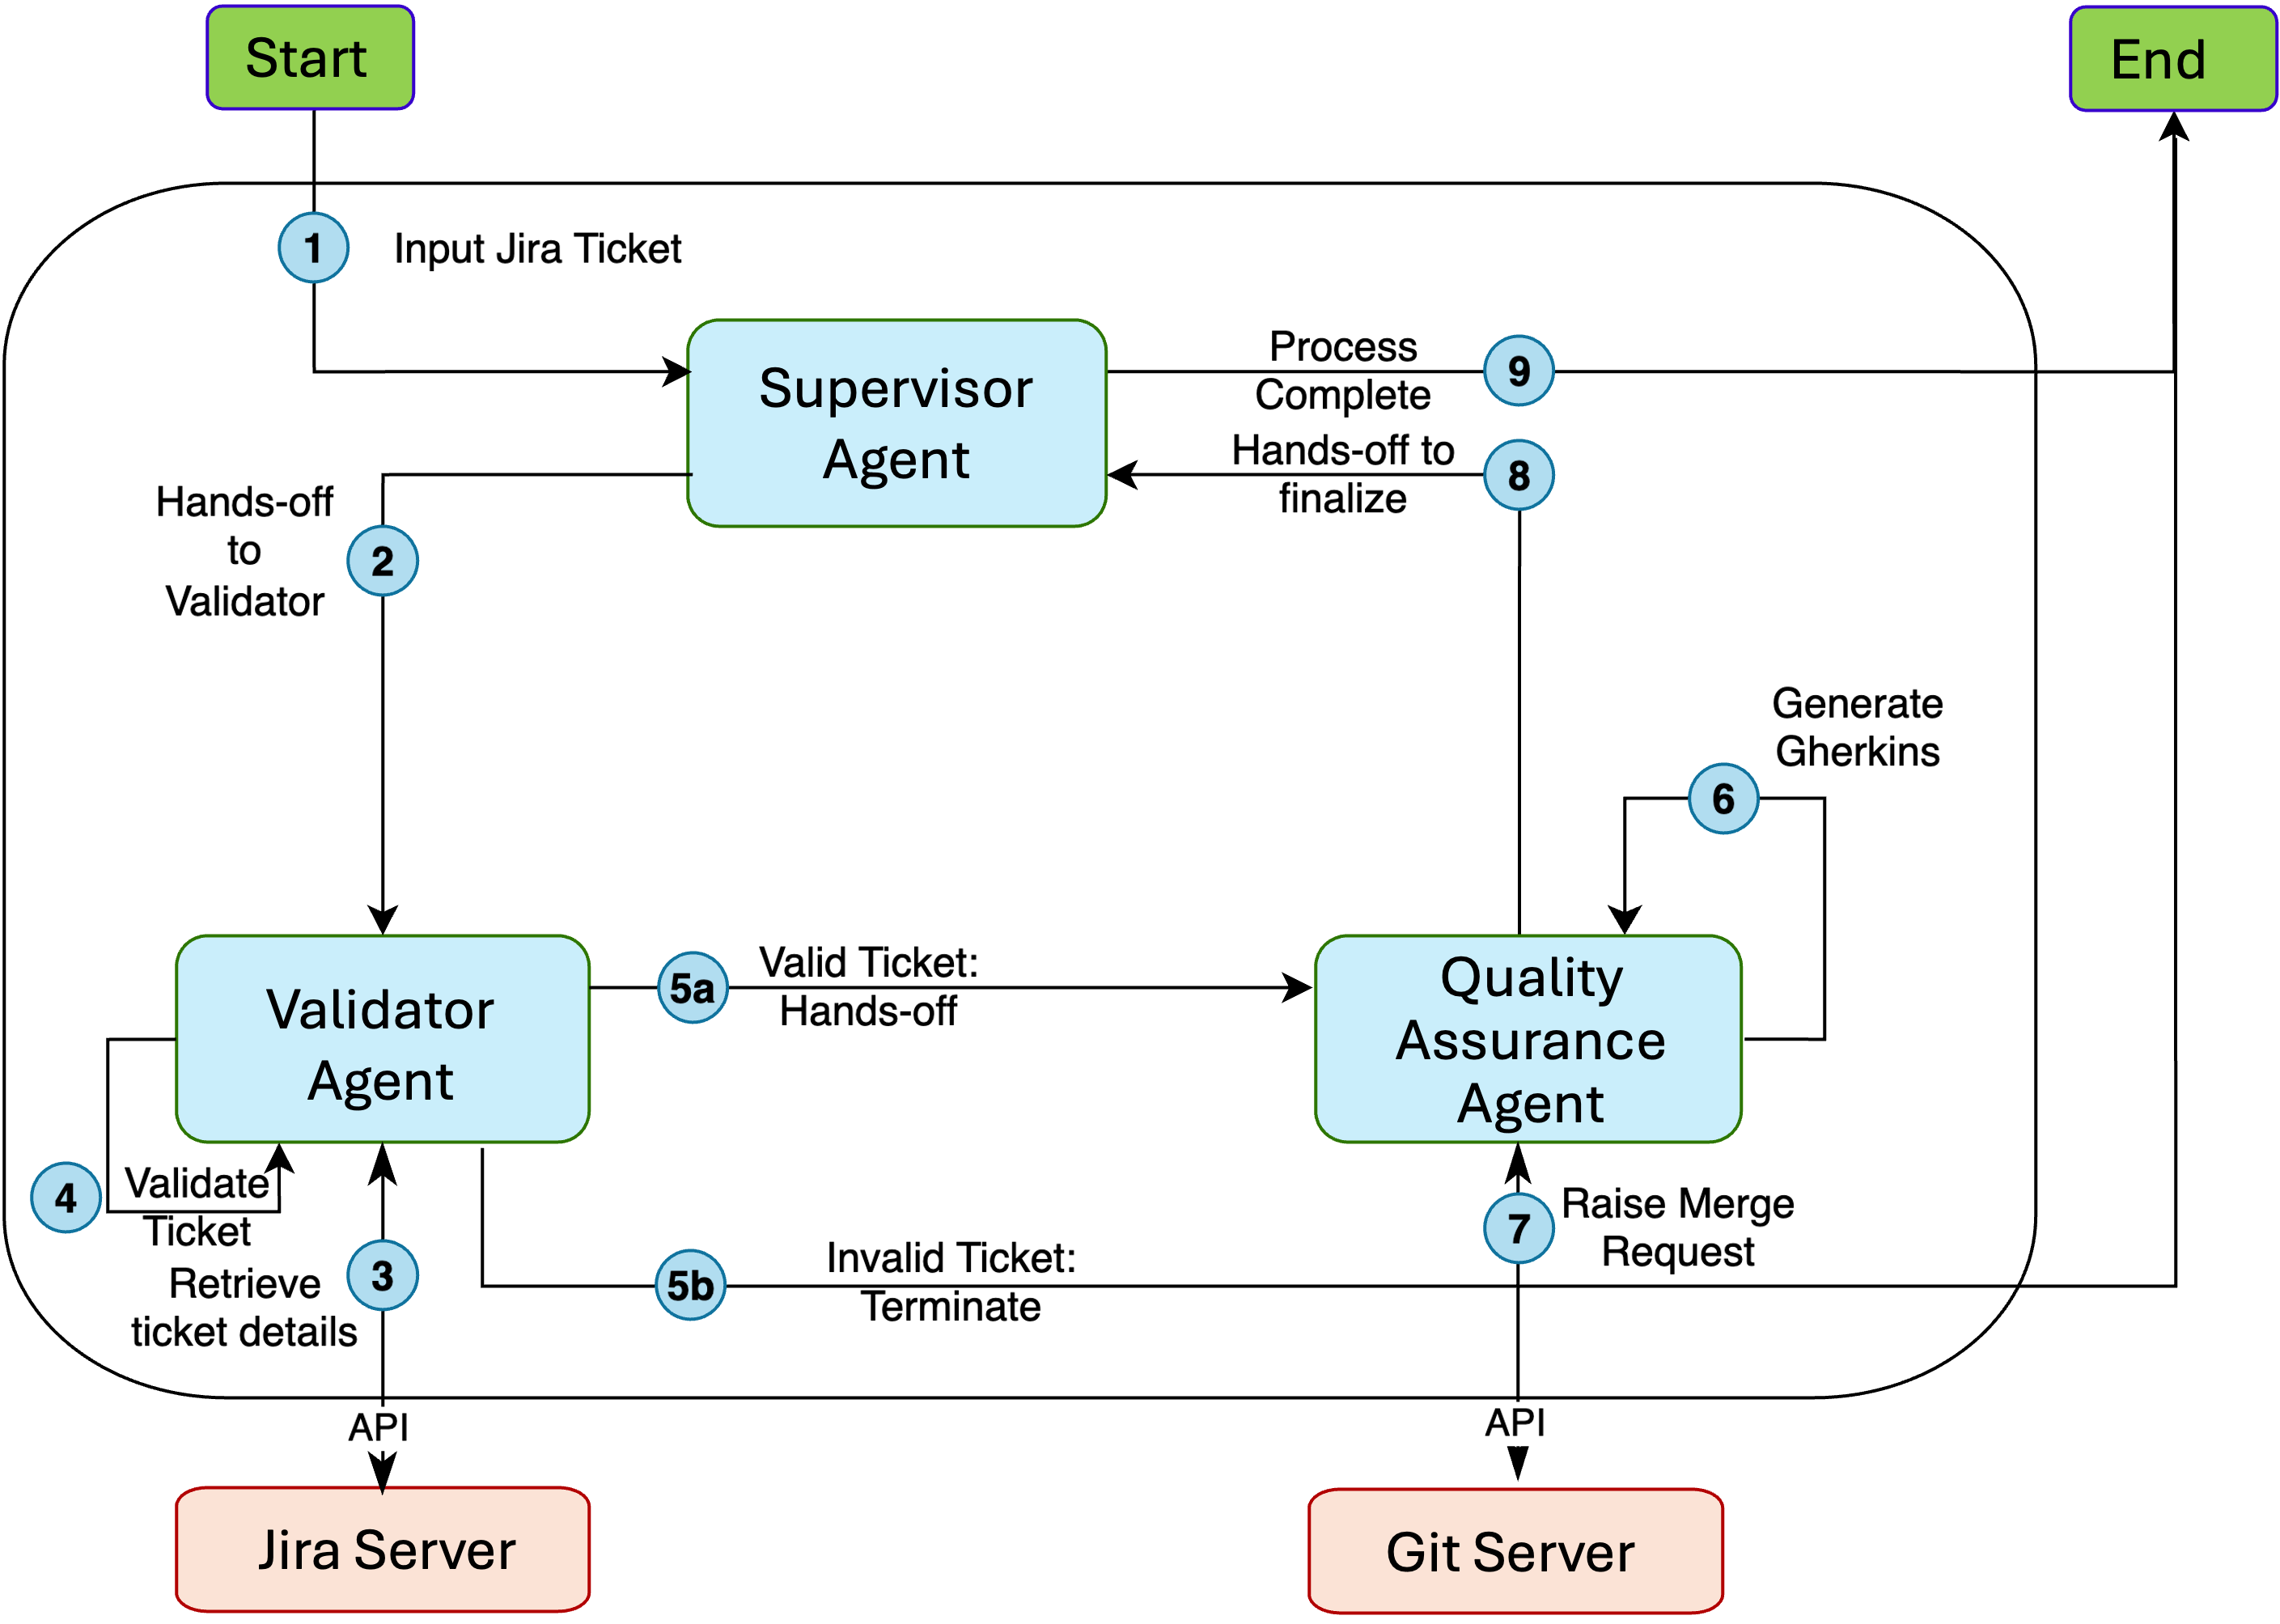
\includegraphics[width=\linewidth]{figures/architecture-v5.png}
\caption{
Architecture and operational workflow of the proposed CMAS4G2 --- a cooperative multi-agent LLM system for automated Gherkin acceptance test generation.
The diagram illustrates the nine-step process, highlighting the roles of the agents (Supervisor, Validator, and Quality Assurance), their interactions, and external API integrations with Jira and Git servers.
}
\label{fig:MAS-design}
\end{figure}

The CMAS4G2 framework comprises three specialized agents as shown in Figure~\ref{fig:MAS-design}:
\begin{itemize}
\item \textbf{Supervisor Agent}: Orchestrates the overall workflow, managing handoffs between agents, monitoring process states, and handling error conditions.
\item \textbf{Validator Agent}: Retrieves ticket details via Jira API and validates requirement completeness, acceptance criteria clarity, and technical feasibility before approving test generation.
\item \textbf{Quality Assurance Agent}: Transforms validated requirements into executable Gherkin acceptance tests and integrates with Git for automated merge request creation.
\end{itemize}

The architecture is extensible, supporting the addition of new agents or human feedback mechanisms. The system implements a sequential workflow with conditional branching across four phases:

\noindent\textbf{Initialization} (Steps 1--2): The Supervisor receives a Jira ticket identifier and hands off to the Validator.

\noindent\textbf{Validation} (Steps 3--5): The Validator retrieves and validates ticket details. Failed validation triggers a Jira comment and workflow termination.

\noindent\textbf{Generation} (Steps 6--7): The QA Agent generates Gherkin scripts and creates automated merge requests via Git.

\noindent\textbf{Completion} (Steps 8--9): The Supervisor finalizes the process, ensuring all artifacts are committed.

\subsection{Technical Implementation Details}
\noindent \textbf{AutoGen Swarm Implementation.}
The CMAS4G2 is implemented using Microsoft AutoGen's Swarm framework, which provides a robust foundation for orchestrating conversational agents with structured handoff mechanisms~\cite{autogen_swarm_docs,autogen_handoffs}. Our implementation leverages AutoGen's native capabilities for agent coordination, tool integration, and termination condition management.

\noindent \textbf{Agent Configuration.}
The following outlines each agent's key configuration. For brevity, only prompt excerpts are shown; full prompt templates are available in the open-source repository.
\begin{itemize}
  \item \textbf{Supervisor Agent}: Configured with zero temperature to ensure deterministic coordination decisions. Equipped with process-monitoring capabilities and the ability to recognize termination signals.
    \textbf{Prompt:}
    \begin{minted}[fontsize=\scriptsize, breaklines, frame=single]{text}
You are the supervisor agent for the Quality Guardian swarm. The validator agent will validate the Jira ticket and provide validation results. The Quality Assurance agent will generate a Gherkin script based on the validation results. Your role is to oversee the process and ensure that the agents are working correctly. You do not need to take any actions, just monitor the process.
<details omitted for brevity>
    \end{minted}
  \item \textbf{Validator Agent}: Operates with zero temperature to guarantee consistent validation logic. Designed for binary decision-making with explicit handoff targets.
\textbf{Prompt:}
\begin{minted}[fontsize=\scriptsize, breaklines, frame=single]{text}
You are a Validator Agent responsible for verifying whether a provided Jira Ticket contains sufficient and correct information
Your role is to:
- Validate the ticket's completeness and correctness
- Save the validation results
- Decide what to do next based on the result:
  - Handoff to the Quality Assurance Agent (if VALID)
  - Use QUALITY_GUARDIAN_QUALITY_ANALYSIS_FAILED to TERMINATE the process IMMEDIATELY (if INVALID)
<details omitted for brevity>
\end{minted}
  \item \textbf{Quality Assurance Agent}: Operates with a moderate temperature (0.6) to encourage comprehensive Gherkin scenario generation while preserving structural consistency. Equipped with repository-integration tools for automated artifact management and capable of handing off to the Supervisor for process completion.
\textbf{Prompt:}
\begin{minted}[fontsize=\scriptsize, breaklines, frame=single]{text}
You are an expert quality assurance engineer with deep experience in creating Gherkin scripts for user acceptance tests.
Your role is to:
- Manually generate a detailed Gherkin script that covers **all possible combinations** of use cases based on the ticket
- Save the generated script
- Provide the saved link to the user
- After you call the `save_script` tool, handoff to the supervisor agent to finalize.
<details omitted for brevity>
\end{minted}
\end{itemize}
\noindent \textbf{Handoff Orchestration.}
The system implements structured handoff mechanisms using AutoGen's native \texttt{Handoff} objects, enabling seamless agent transitions with contextual information preservation. The Validator Agent employs conditional handoff logic based on validation outcomes: successful validation triggers handoff to the Quality Assurance Agent, while validation failures invoke immediate process termination.

% [RESPONSE R2-W1] Clarify syntactic Gherkin validation and its scope (reviewer asked about
% gherkin-lint / parser / execution checks). See review-responses.md § R2-W1 and R2-Q1.
\noindent \textbf{Gherkin Syntactic Validation.}
Before committing, the system runs \texttt{is\_valid\_gherkin()}, requiring a \texttt{Feature:} block, at least one \texttt{Scenario:} declaration, and at least one step keyword; failing files are counted as failures. This structural check does not cover \texttt{gherkin-lint} or execution against live BDD runners (a limitation noted in Section~\ref{sec:conclusion}).

\noindent \textbf{Tool Integration Framework.}
Beyond the Supervisor agent, each agent maintains access to specialized tool sets that enable parameterized tool calls with ticket-specific context. The Validator Agent integrates with Jira APIs for ticket retrieval and comment creation. The Quality Assurance Agent interfaces with version control systems through Git APIs, enabling automated merge request creation and script artifact management. To support automated benchmarking, both agents support file-based operations in benchmark mode.

\noindent \textbf{Model Integration and Infrastructure.}
The system integrates both open-weight and proprietary LLMs through a unified OpenAI-compatible API interface, ensuring consistent reasoning and generation capabilities across agents. This standardized approach simplifies integration across model families while preserving uniform interaction patterns.
Our evaluation focuses on two families of open-weight models with demonstrated performance in code generation and reasoning tasks:

\begin{itemize}
  \item \textbf{Qwen3 Family:} Three parameter scales (8B, 14B, 32B), tested under both direct inference (\textit{no\_think}) and structured reasoning (\textit{think}) modes.
  \item \textbf{GPT-OSS (20B):} Tested under three reasoning intensities---low, medium, and high---reflecting progressively deeper chain-of-thought generation. The larger 120B variant was excluded due to hardware constraints.
\end{itemize}

These models are executed locally via LM Studio\footnote{\url{https://lmstudio.ai/}} with an 8192-token context window on an \textbf{NVIDIA GeForce RTX~4090 GPU} (24\,GB VRAM), representative of a high-end developer workstation.
For comparison, we evaluate \textbf{Claude Sonnet~4} through Anthropic's OpenAI-compatible API\footnote{\url{https://docs.claude.com/en/api/openai-sdk}}, serving as a proprietary state-of-the-art baseline under identical conditions.

\subsection{Dataset Benchmark}
To systematically evaluate the CMAS4G2 framework, we curated a comprehensive benchmark dataset based on the open-source Kill Bill subscription billing and payments platform\footnote{\url{https://github.com/killbill}}. This platform provides both authenticity and real-world relevance, as it is a production-grade system with an extensive API surface and the kind of complex business logic typical of enterprise software applications.

\noindent \textbf{Dataset Construction Methodology.}
The dataset comprises 200 synthetic Jira tickets crafted by experienced QA engineers with Kill Bill domain expertise, following a consistent structure that mirrors realistic enterprise development scenarios.

\noindent \textbf{Dataset Composition and Validation Criteria.}
The dataset maintains realistic distribution across HTTP methods, reflecting typical API usage patterns:
\begin{itemize}
\item GET: 100 tickets (50\%) --- covering data retrieval scenarios
\item POST: 42 tickets (21\%) --- focusing on resource creation workflows
\item DELETE: 30 tickets (15\%) --- addressing resource removal scenarios
\item PUT: 28 tickets (14\%) --- covering resource update operations
\end{itemize}

% [RESPONSE R2-W2] Expanded invalid ticket construction to explain the paired structure and
% specific element omissions. See review-responses.md § R2-W2.
\noindent \textbf{Validity Classification Framework.}
The dataset implements a balanced binary structure: 100 valid tickets (IDs 1--100) and 100 invalid tickets (IDs 101--200).
Valid tickets contain all mandatory elements:
\begin{itemize}
\item \textbf{Descriptive Title}: Clear, concise identification of the API functionality being tested.
\item \textbf{Comprehensive Description}: Detailed specification of the API endpoint, including expected behavior and business logic context, typed path/query/header parameters, and request body schemas where applicable.
\item \textbf{Acceptance Criteria}: Structured requirements defining the scope and boundaries of the functionality.
\item \textbf{Success Scenarios}: Explicit definition of positive test cases with expected HTTP status codes and response formats.
\item \textbf{Error Scenarios}: Comprehensive coverage of failure modes, edge cases, and exception handling requirements (e.g., 400/404/500 conditions).
\end{itemize}
Invalid tickets (IDs 101--200) are \emph{paired counterparts} of the valid tickets, targeting the same API endpoints but retaining only a minimal description (2--3 sentences) and a partial acceptance criterion (typically just the primary success status code), while omitting parameter specifications, request body schemas, and error scenarios. This paired structure forces genuine \emph{semantic} completeness analysis rather than superficial keyword detection.

\subsection{LLM-as-a-Judge Evaluation}
\label{sec:llm-as-a-judge}
% [RESPONSE R1-W1] Added explicit acknowledgment of the LAJ-vs-human limitation and the
% calibration evidence. See review-responses.md § R1-W1.
To objectively and scalably assess the test coverage of Gherkin scripts generated by CMAS4G2, we adopt the \emph{LLM-as-a-Judge} (LAJ) evaluation framework proposed by Huang et al.~\cite{huang2025laj}. LAJ provides an automated, rubric-driven procedure that reads a ticket description, the corresponding generated Gherkin script, and a concise evaluation rubric, then returns a structured coverage percentage and rationale. The framework was validated to achieve elite-level accuracy in aligning with expert human judgments while enabling high-throughput, cost-effective evaluation.

% [RESPONSE R2-Q2] Added rubric component details (system role, user inputs, output schema).
% See review-responses.md § R2-Q2.
The judge is prompted as a senior BDD QA engineer; its input combines the full Jira story, the generated Gherkin file, and Kill Bill API testing guidelines. The structured JSON output includes \texttt{coverage\_percentage} (0--100), \texttt{covered}, \texttt{gaps}, and \texttt{recommendations}; no per-criterion weights are assigned.

Following the comprehensive calibration analysis in~\cite{huang2025laj}, we selected \textbf{GPT-4o Mini} as the judge model (temperature~$= 0$), providing near-best-in-class accuracy (Mean Absolute Assessment Error of 6.29~pp relative to expert human annotators) at substantially reduced cost. This paper does not include an independent human evaluation; alignment with human judgement is inherited from~\cite{huang2025laj}, with domain-specific spot-checks left as future work.

\subsection{CMAS4G2 Performance Evaluation}
\label{sec:eval-metrics}
% [RESPONSE R2-Q1] Clarified Valid SR definition: non-empty, structurally valid Gherkin file
% committed to Git. See review-responses.md § R2-Q1.
We assess CMAS4G2 performance across four complementary metrics,
each capturing a distinct aspect of system effectiveness:
\begin{itemize}
\item \textbf{Valid Ticket Success Rate (Valid SR):}
Percentage of valid tickets (IDs 1--100) for which the system produces and commits a structurally valid Gherkin file (passing \texttt{is\_valid\_gherkin()}) via an automated merge request.
\item \textbf{Invalid Ticket Success Rate (Invalid SR):}
Percentage of invalid tickets (IDs 101--200) correctly rejected before test generation, with a Jira comment posted and the workflow terminated.
\item \textbf{Overall Success Rate (Overall SR):}
Combined success across all 200 tickets: $\text{Overall SR} = (\text{Valid SR} + \text{Invalid SR})/2$.
\item \textbf{Average Test Coverage (Avg Coverage):}
Mean coverage score assigned by the LAJ framework (Section~\ref{sec:llm-as-a-judge}) for successfully generated scripts, reflecting semantic alignment with ticket acceptance criteria.
\end{itemize}
\section{Results and Discussions}
\label{sec:results}
We evaluate all CMAS4G2 configurations across the 200-ticket benchmark using GPT-4o Mini as the LLM-as-a-Judge, selected based on the comprehensive calibration study in~\cite{huang2025laj}. The evaluation systematically varies model families, scales, and reasoning modes.

% \subsection{CMAS4G2 Performance Analysis}
% \label{sec:model-performance}
Table~\ref{tab:cmas4g2_performance} presents comprehensive performance metrics across all evaluated model configurations, organized by model family and systematically varying capacity and reasoning modes. All metrics are reported as mean $\pm$ standard deviation across five independent evaluation runs to characterize performance stability and reproducibility.

\begin{table}[htbp]
\centering
\caption{CMAS4G2 Performance Evaluation: Success Rates and Test Coverage Across Model Configurations}
\label{tab:cmas4g2_performance}
\small
\setlength{\tabcolsep}{3pt}
\begin{tabular}{@{}llcccc@{}}
\toprule
\textbf{Model} & \textbf{Config.} & \textbf{Valid SR} & \textbf{Invalid SR} & \textbf{Overall SR} & \textbf{Avg Cov.} \\
 & & \textbf{(\%)} & \textbf{(\%)} & \textbf{(\%)} & \textbf{(\%)} \\
\midrule
\multirow{6}{*}{Qwen3} & 8B (no\_think) & 58.80$\pm$24.42 & 41.00$\pm$0.00 & 49.90$\pm$12.21 & 79.48$\pm$3.10 \\
 & 8B (think) & 98.00$\pm$1.55 & 57.00$\pm$0.00 & 77.50$\pm$0.77 & 79.18$\pm$0.34 \\
 & 14B (no\_think) & 89.20$\pm$2.48 & 58.00$\pm$0.00 & 73.60$\pm$1.24 & 81.90$\pm$1.00 \\
 & 14B (think) & 84.40$\pm$3.38 & 44.00$\pm$0.00 & 64.20$\pm$1.69 & 74.73$\pm$4.76 \\
 & 32B (no\_think) & \textbf{99.20$\pm$1.17} & 35.20$\pm$0.40 & 67.20$\pm$0.60 & \textbf{86.91$\pm$0.42} \\
 & 32B (think) & 87.20$\pm$4.66 & \textbf{69.00$\pm$0.00} & \textbf{78.10$\pm$2.33} & 83.67$\pm$0.26 \\
\midrule
\multirow{3}{*}{GPT-OSS} & 20B (low) & 96.40$\pm$1.85 & \textbf{76.80$\pm$0.40} & 86.60$\pm$0.80 & \textbf{85.72$\pm$0.23} \\
 & 20B (medium) & \textbf{99.20$\pm$1.60} & 76.00$\pm$0.00 & \textbf{87.60$\pm$0.80} & 85.39$\pm$0.28 \\
 & 20B (high) & 1.60$\pm$3.20 & 73.00$\pm$0.00 & 37.30$\pm$1.60 & 16.75$\pm$33.50 \\
\midrule
Claude & Sonnet 4 & \textbf{100.00$\pm$0.00} & \textbf{80.80$\pm$0.40} & \textbf{90.40$\pm$0.20} & \textbf{91.57$\pm$0.22} \\
\bottomrule
\end{tabular}
\vspace{4pt}
\noindent\footnotesize
SR: Success Rate; Valid SR: successful generation rate on valid tickets (IDs 1--100); Invalid SR: successful rejection rate on invalid tickets (IDs 101--200); Overall SR: combined performance across all 200 tickets; Avg Cov.: mean test coverage percentage for successfully generated scripts. All metrics represent mean $\pm$ standard deviation across 5 independent evaluation runs. Bold values indicate best performance per model family.
\end{table}

\subsection{Overall Performance Hierarchy.}
Claude Sonnet 4 establishes the performance ceiling with 90.4\% ($\pm$0.2\%) overall success and 91.57\% ($\pm$0.22\%) coverage as shown in Table~\ref{tab:cmas4g2_performance}. Among open-weight models, GPT-OSS 20B (medium) achieves the strongest performance with 87.6\% ($\pm$0.8\%) success and 85.39\% ($\pm$0.28\%) coverage, approaching within 2.8 percentage points of the proprietary baseline while enabling fully local deployment. GPT-OSS 20B (low) follows closely with 86.6\% ($\pm$0.8\%) success and 85.72\% ($\pm$0.23\%) coverage.
The Qwen3-32B (think) achieves 78.1\% ($\pm$2.33\%) overall success with 83.67\% ($\pm$0.26\%) coverage, while Qwen3-8B (think) reaches 77.5\% ($\pm$0.77\%) with 79.18\% ($\pm$0.34\%) coverage. Coverage percentages vary widely (17--92\%), with thinking mode, model scale, and reasoning intensity playing critical roles.

\subsection{Valid Ticket Processing Performance.}
\label{sec:valid-ticket-processing}
Claude Sonnet 4 achieves perfect 100\% success rate. Among open-weight models, both Qwen3-32B (no\_think) and GPT-OSS 20B (medium) achieve 99.2\%, with Qwen3-32B at $\pm$1.17\% and GPT-OSS 20B (medium) at $\pm$1.60\% standard deviation, nearly matching Claude's performance. GPT-OSS 20B (low) follows at 96.4\% ($\pm$1.85\%).

As shown in Table~\ref{tab:cmas4g2_performance}, the Qwen3 family exhibits scale-dependent reasoning effects. The 8B model shows dramatic improvement with thinking mode: from 58.8\% ($\pm$24.42\%) to 98.0\% ($\pm$1.55\%)---a 39.2 percentage point gain with substantially reduced variance. The 14B configuration reveals a reversal: no\_think achieves 89.2\% ($\pm$2.48\%), outperforming think at 84.4\% ($\pm$3.38\%), suggesting coordination overhead degrades mid-scale performance. The 32B shows further degradation: from 99.2\% ($\pm$1.17\%) without thinking to 87.2\% ($\pm$4.66\%) with thinking---a 12 percentage point drop.

% [RESPONSE R2-Q3] Added context window budget details, token consumption explanation,
% and note on 16k supplementary run. See review-responses.md § R2-Q3.
The GPT-OSS family reveals a sharp reasoning intensity threshold. Medium reasoning achieves 99.2\% ($\pm$1.60\%) valid success---matching the highest performance among open-weight models---and low reasoning follows at 96.4\% ($\pm$1.85\%). High reasoning, however, exhibits catastrophic failure at 1.6\% ($\pm$3.2\%)---a 97.6~pp collapse from medium. Execution logs show that high-reasoning chain-of-thought generation exhausts the 8,192-token context window (shared by conversation history, tool call results, and reasoning tokens) before the \texttt{save\_script} tool call fires, yielding empty API responses and Supervisor-triggered workflow termination. A supplementary run at 16,384 tokens (\texttt{gpt-oss-20b\_16k\_high}), executed on an Nvidia RTX~A6000 (48\,GB VRAM), confirms the diagnosis: expanding the context budget fully restores normal performance.

\subsection{Invalid Ticket Rejection Performance.}
Claude Sonnet 4 achieves 80.8\% ($\pm$0.4\%) rejection rate. The GPT-OSS family shows stable rejection across reasoning intensities: 76.8\% ($\pm$0.4\%) (low), 76.0\% (medium), and 73.0\% (high)---contrasting sharply with catastrophic valid ticket failures at high reasoning. This suggests validation decisions occur early in the workflow before extensive context consumption.
The Qwen3 family exhibits inconsistent rejection behavior. The 8B improves from 41.0\% (no\_think) to 57.0\% (think)---a 16 percentage point gain. The 14B unexpectedly decreases from 58.0\% to 44.0\%---a 14 percentage point drop. The 32B shows dramatic improvement: from 35.2\% ($\pm$0.4\%) to 69.0\% (think)---a 33.8 percentage point increase. This creates a paradox where thinking mode degrades valid processing (99.2\% to 87.2\%) while improving invalid rejection (35.2\% to 69.0\%), suggesting explicit reasoning shifts behavior toward conservative validation.

\subsection{Test Coverage Quality Analysis.}
Coverage is consistently high (75--92\%) across most configurations when workflows complete successfully, with narrow standard deviations ($<$1\%) indicating stable generation. Claude Sonnet 4 leads at 91.57\% ($\pm$0.22\%), followed by Qwen3-32B (no\_think) at 86.91\% ($\pm$0.42\%) and GPT-OSS 20B (low) at 85.72\% ($\pm$0.23\%). GPT-OSS 20B (medium) achieves 85.39\% ($\pm$0.28\%) with excellent stability, while Qwen3-32B (think) reaches 83.67\% ($\pm$0.26\%).

% Thinking mode primarily improves consistency rather than absolute coverage for smaller models: Qwen3-8B achieves similar averages ($\sim$79\%) but 9.1$\times$ lower variance with thinking enabled. 
% FIX 2
Thinking mode primarily improves consistency rather than absolute coverage for smaller models: Qwen3-8B achieves similar averages ($\sim$79\%) but 9.1$\times$ lower \textit{coverage} variance with thinking enabled (standard deviation: 3.10\% $\to$ 0.34\%).
The 14B (think) attains 74.73\% ($\pm$4.76\%), the lowest among successfully completing workflows. GPT-OSS 20B (high) is the notable exception, achieving only 16.75\% ($\pm$33.50\%) due to context exhaustion as discussed in Section~\ref{sec:valid-ticket-processing}.

\section{Conclusion}
\label{sec:conclusion}
This paper demonstrated that \textbf{CMAS4G2}, a cooperative multi-agent system for automated Gherkin acceptance test generation, achieves performance approaching proprietary alternatives using locally deployed open-weight models on consumer hardware. Our key outcomes include: (1)~a production-ready multi-agent architecture using AutoGen Swarm that coordinates specialized agents for requirement validation, test generation, and quality assurance; (2)~empirical evidence that GPT-OSS 20B (medium) reaches 87.6\% ($\pm$0.8\%) success and 85.39\% ($\pm$0.28\%) coverage versus Claude Sonnet 4's 90.4\% ($\pm$0.2\%) and 91.57\% ($\pm$0.22\%), a gap of only 2.8~pp; and (3)~demonstration that reasoning configuration profoundly impacts performance: structured reasoning enables transformative gains for small models (Qwen3-8B: +27.6~pp overall success, 15.7$\times$ lower \textit{Valid SR} variance: 24.42\% $\to$ 1.55\%), while excessive depth causes catastrophic failure through context exhaustion (GPT-OSS 20B high: 37.3\% success). Test coverage was assessed using the LLM-as-a-Judge framework~\cite{huang2025laj}.

% [RESPONSE R1-W2] Frame the small gap (2.8 pp) as a positive viability finding, distinguishing
% it from the catastrophic GPT-OSS high case. See review-responses.md § R1-W2.
% [RESPONSE R2-W1-FW] Add execution-level validation as explicit future work. See review-responses.md § R2-W1.
% [RESPONSE R2-Q3] Add context-budget deployment guidance. See review-responses.md § R2-Q3.
CMAS4G2 advances the democratization of AI-powered testing, making enterprise-grade automation accessible without cloud dependencies or prohibitive cost. The 2.8~pp gap to the proprietary baseline (Claude Sonnet~4) is a \emph{positive} finding: local deployment on consumer hardware achieves near-parity quality, and the catastrophic failures at high reasoning depth (GPT-OSS~20B high: 37.3\%) are fully explainable and avoidable through appropriate context-window configuration. Practitioners should nonetheless view CMAS4G2 as an augmentation tool that accelerates routine test creation rather than a replacement for human expertise in requirements engineering and edge case identification.

Several limitations and future directions merit attention. \textbf{Execution-level validation:} our current success criterion covers only structural (syntactic) validity; future work should validate executability against a live BDD runner (e.g., Cucumber-JVM, Reqnroll) with auto-generated step definitions and a Kill Bill sandbox. \textbf{Human evaluation:} an independent spot-check on a sample of generated scripts would complement the LAJ-based coverage scores. \textbf{Context management:} deployments using high-reasoning modes should configure context budgets and consider summarization or external memory to prevent exhaustion. Further extensions include broader domains (microservices, event-driven architectures), ambiguous and underspecified tickets, additional BDD frameworks (SpecFlow, Behave) and CI/CD platforms, and diverse hardware (Apple Silicon, AMD GPUs) with quantization and energy profiling.

%%%%%%%%%%%%%%%%%%%%%%%%%%%%%%%%%%%%%%%%%%%%%%%%%%%%%%%%%%%%%%%%%%%%%%%%
\iffalse
\begin{credits}
\subsubsection{\ackname}
We acknowledge the support of our research institutions and the open-weight community for providing the foundational tools and datasets that enabled this research.
\end{credits}
\fi
%%%%%%%%%%%%%%%%%%%%%%%%%%%%%%%%%%%%%%%%%%%%%%%%%%%%%%%%%%%%%%%%%%%%%%%%
\bibliographystyle{splncs04}
\bibliography{references}
\end{document}
